\documentclass[xcolor={cmyk}]{beamer}
\usepackage[utf8]{inputenc}
\usepackage[T1]{fontenc}
\usepackage[english]{babel}
% \graphicspath{{./pics/}}

\title{Design of Adversarial Inputs for Deep Neural\\ Networks using Iterative Approximations}
\subtitle{Entwurf bösartiger Eingaben für tiefe neuronale Netze\\mittels iterativer Approximationen}
\author[Philipp Braun]{Philipp Braun\\
\footnotesize{\texttt{philipp.braun@rwth-aachen.de}}}
\date{\today}

% Select theme
\usetheme[english]{RWTH_Ti}
% oder
% \usetheme[german]{RWTH_Ti}
% passt den Institutsnamen an.
%Wenn bable entsprechend gesetzt ist, wird sich auch das Datumsformat ändern.

\usepackage{graphicx}
\usepackage{amsmath}
\usepackage{latexsym}                % wegen \Box
\usepackage{dsfont}                  % wegen mathematische notation von mengensymbole
\usepackage{mathtools}               % wegen erweiterte mathematische notation, vorallem aber f\"{u}r das mathematische definitionszeichen
\usepackage{xcolor}                  % wegen incscape, um gute grafiken zu erstellen
\usepackage{subfigure}
\usepackage{pgf}
\usepackage{pgfpages}

% \usepackage{algorithm,algpseudocode}
\usepackage{algorithm,algorithmic}


\setlength{\doublerulesep}{0pt}
\usepackage{multirow} % Multirows in tabulars
\usepackage{longtable, tabu} % Flexible tabulars i.e. page breaks and horizontal fill
\newtabulinestyle{mydashline=on 1.5pt off 2pt}
\tabulinesep=1mm

\usepackage{lmodern}
% \usepackage[style=ieee,backend=biber]{biblatex}
% \addbibresource{\jobname.bib}
\setbeamerfont{footnote}{size=\tiny}

\newcommand{\mbf}{\mathbf}
\newcommand{\mbb}{\mathbb}
\newcommand{\mcl}{\mathcal}
\newcommand{\mrm}{\mathrm}
\newcommand{\bm}{\boldsymbol}
\newcommand{\real}{\mathbb{R}}
\newcommand{\ma}[1]{{\mathbf #1}}
\DeclareMathOperator*{\argmin}{argmin}
\DeclareMathOperator*{\argmax}{argmax}
\newtheorem{proposition}{Proposition}
\newtheorem{remark}{Remark}

\graphicspath{{./figures/}}

\begin{document}

% Titlepage
\frame[plain]{\titlepage}

\AtBeginSection[]
{
	\begin{frame}[plain, noframenumbering]
		\frametitle{Table of Contents}
		\tableofcontents[
		    currentsubsection,
			sectionstyle=show/shaded,
			subsectionstyle=show/shaded,
		]
	\end{frame}
}

\AtBeginSubsection[]
{
	\begin{frame}[plain, noframenumbering]
		\frametitle{Table of Contents}
		\tableofcontents[
		    currentsubsection,
			sectionstyle=show/shaded,
			subsectionstyle=show/shaded,
			subsubsectionstyle=show/shaded,
		]
	\end{frame}
}

\AtBeginSubsubsection[]
{
	\begin{frame}[plain, noframenumbering]
		\frametitle{Table of Contents}
		\tableofcontents[
		    currentsubsection,
			sectionstyle=show/shaded,
			subsectionstyle=show/shaded,
			subsubsectionstyle=show/shaded,
		]
	\end{frame}
}

\begin{frame}{Table of Contents}
\tableofcontents
\end{frame}



% --------------------------------------- Introduction ---------------------------------------
\section{Introduction}
\begin{frame}{Overview}{Introduction}
	\begin{itemize}
		\item DNNs have been popularized for image classfication tasks and a multitude of regression problems
		\item System failures in medical applications or autonomous driving can be fatal
		\item Proper techniques to analyze the failure of these systems are necessary
	\end{itemize}
\end{frame}

\begin{frame}{Motivation}{Introduction}
	Adversarial attacks can be implemented in the real world using stickers and graffitis \footnote{Kevin Eykholt, Ivan Evtimov, Earlence Fernandes and Bo Li, "Robust Physical-World Attacks on Deep Learning Visual Classification", https://arxiv.org/pdf/1707.08945.pdf}
	\begin{figure}
	\centering
	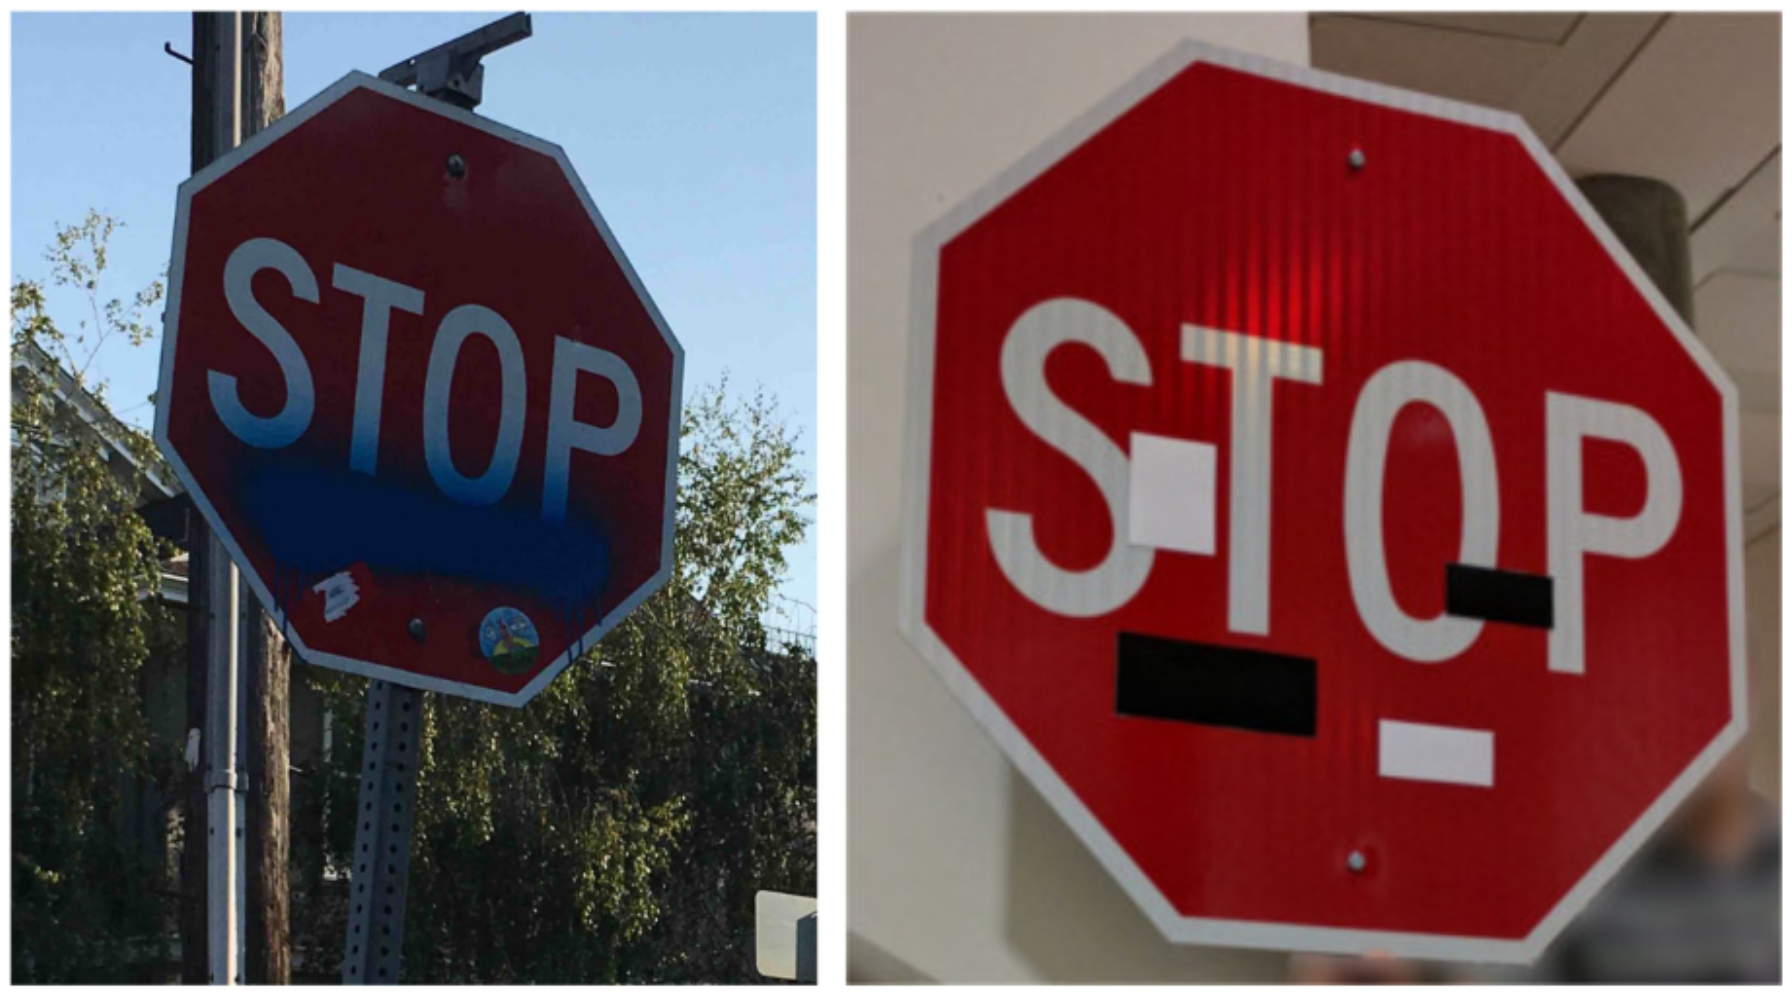
\includegraphics[scale=0.3]{street-adversarial}
	\end{figure}
\end{frame}


\begin{frame}{Previous Work}{Introduction}
	Adversarial attacks for classification tasks have been widely explored. Examples include

	\begin{itemize}
		\item DeepFool\footnote{Seyed-Mohsen Moosavi-Dezfooli, Alhussein Fawzi, Pascal Frossard, "DeepFool: a simple and accurate method to fool deep neural networks", https://arxiv.org/pdf/1511.04599.pdf}
		\item Fast Gradient-Sign Method (FGSM)\footnote{Ian J. Goodfellow, Jonathon Shlens \& Christian Szegedy, "Explaining and Harnessing Adversarial Examples", https://arxiv.org/pdf/1412.6572.pdf}
	\end{itemize}

	Little research has been done into regression problems and autoencoders
\end{frame}


\section{Regression Problem}
\begin{frame}{Regression Problem}

	\begin{itemize}
		\item $\bm{x}$ denotes the input,
		\item $\bm{y}$ denotes the output,
		\item $f(\bm{x}) \approx \bm{y}$ describes the model's function,
		\item $\bm{\eta}$ denotes the adversarial perturbation\\[10pt]
	\end{itemize}

	\begin{definition}
	\begin{itemize}
		\item $ N \in  \mathbb{N} $ samples are drawn from a set of samples $ \{(\bm{x}_i, \bm{y}_i)\}^N_{i=1} $
		using an unknown distribution $ P_{X,Y} $
		\item Regression model computes a function that minimizes the loss $ \mcl{L}(f(\bm{x}), \bm{y}) = \lvert\lvert f(\bm{x}) - \bm{y} \rvert\rvert^2_2 $
	\end{itemize}
	\end{definition}
\end{frame}


\begin{frame}{Adversarial Examples}{Introduction}

	\begin{itemize}
		\item $p > 1$ is used in the $\ell_p$-norm
		\item A small $\bm{\eta}$ maximizes the error of $f(\bm{x} + \bm{\eta})$
		\item $\epsilon \in \mathbb{R}_{+}$ constrains the input perturbation\\[20pt]
	\end{itemize}

	The goal of an attacker is given by
	\begin{equation*}
	\begin{aligned}
		\max_{ \bm{\eta} } \; \mcl{L}(\bm{x} + \bm{\eta}) = \max_{ \bm{\eta} } \; \lvert\lvert f(\bm{x} + \bm{\eta}) - \bm{y} \rvert\rvert^2_2 \quad \text{s.t.} \quad \lvert\lvert \bm{\eta} \rvert\rvert_p  \leq \epsilon \\
	\end{aligned}
	\end{equation*}\\[10pt]

	This problem is non-convex and non-linear since it depends on the model's function $f$. Therefore, we cannot easily solve it.

\end{frame}


\section{Linear Programming Problem}
\begin{frame}{Taylor Approximation}{Linear Programming Problem}
	To create a solvable maximization problem, we linearize $\mcl{L}$ using a first order taylor expansion.

	\begin{equation*}
	\begin{aligned}
		\mcl{L}(\bm{x} + \bm{\eta}) &\approx \mcl{L}(\bm{x}) + \bm{\eta}^T \nabla \mcl{L}(\bm{x})
	\end{aligned}
	\end{equation*}\\[10pt]

	A maximization problem is then formulated by\\[10pt]

	\begin{equation*}
	\begin{aligned}
		\max \; \bm{\eta}^T \nabla \mcl{L}(\bm{x}) \quad \text{s.t.} \quad \lvert\lvert \bm{\eta} \rvert\rvert_p \leq \epsilon
	\end{aligned}
	\end{equation*}

\end{frame}

\begin{frame}{General Closed-Form Solution}{Linear Programming Problem}

	A closed-form solution for classfication is provided by Balda et al.\footnote{Emilio Rafael Balda, Arash Behboodi, Rudolf Mathar, "On Generation of Adversarial Examples using Convex Programming", 52th Asilomar Conference on Signals, Systems, and Computers}.
	We define $q \triangleq \frac{p}{p-1}$ with $p=2$ or $p=\infty$. $\lvert \nabla \mcl{L}(\bm{x}) \rvert^{q-1}$ provides a vector of the absolute values to the power of $q - 1$.

	\begin{equation*}
	\begin{aligned}
		\bm{\eta} = - \epsilon \frac{1}{\lvert\lvert \nabla \mcl{L}(\bm{x}) \rvert\rvert_q^{q-1}} \cdot ( \text{sign}( \nabla \mcl{L}(\bm{x}) ) \odot \lvert \nabla \mcl{L}(\bm{x}) \rvert^{q-1} )
	\end{aligned}
	\label{linear_programming_solution}
	\end{equation*}

	The same solution is applied to our regression setup and subsequent experiments.

\end{frame}

\begin{frame}{Conditions}{Linear Programming Problem}

	\begin{itemize}
		\item The linear approximation of $\mcl{L}$ is only good if $\bm{\eta}$ is small (usually the case for $\lvert\lvert \bm{\eta} \rvert\rvert_p \leq \epsilon$)
		\item For larger $\epsilon$ we use linear approximations of size $\frac{\epsilon}{N}$ with $N \in \mathbb{N}$
		\item If N is high enough these approximations are good
	\end{itemize}

\end{frame}




\begin{frame}{Iterative Solution}{Linear Programming Problem}

	\begin{algorithm}[H]
	\caption{Iterative Solution for $p = \infty$}
	\begin{algorithmic}[1]
	\STATE \textbf{input:} $\; \bm{x}, f(\bm{x}), \bm{\eta}, N$
	\STATE \textbf{output:} $\; \bm{\eta}$
	\STATE \textbf{initialize:} $\bm{\tilde{x}} \gets \bm{x}$
	\FOR{$i \gets 1, ..., N$}
		\STATE $ \bm{\eta} \gets \frac{\bm{\epsilon}}{N} \; \text{sign}(\nabla \mcl{L}(\bm{\tilde{x}})) $
		\STATE $ \bm{\tilde{x}} \gets \bm{\tilde{x}} + \bm{\eta} $
	\ENDFOR
	\end{algorithmic}
	\end{algorithm}

\end{frame}


\begin{frame}{Perfect Fitting Problem}{Linear Programming Problem}

Solving the loss function using basic algebra shows that linear closed-form solutions
will fail if $\bm{y} = f(\bm{x})$ causing $\nabla \mcl{L} = 0$

	\begin{equation*}
	\begin{aligned}
		\mcl{L}(\bm{x} + \bm{\eta}) &\approx \mcl{L}(\bm{x}) + \bm{\eta}^T \nabla \mcl{L}(\bm{x}) \\[10pt]
			&= \mcl{L}(\bm{x}) + \bm{\eta}^T \nabla( (\bm{y} - f(\bm{x}))^T (\bm{y} - f(\bm{x})) ) \\[10pt]
			&= \mcl{L}(\bm{x}) - 2 \bm{\eta}^T \bm{J}_f(\bm{x}) ( \bm{y} - f(\bm{x}) ) \\[10pt]
	\end{aligned}
	\label{taylorlinear}
	\end{equation*}

\textbf{Solution:} Apply approximation at $\tilde{\bm{x}} \approx \bm{x}$ such that $\nabla \mcl{L} \neq 0$

\end{frame}

\section{Quadratic Programming Problem}

\begin{frame}{Taylor Approximation}{Quadratic Programming Problem}

	Taylor approximation can also be applied on $f(\bm{x})$ inside $\mcl{L}(\bm{x}+\bm{\eta})$

	\begin{equation*}
	\begin{aligned}
	\mcl{L}(\bm{x} + \bm{\eta}) &= \lvert\lvert \bm{y} - f(\bm{x} + \bm{\eta}) \rvert\rvert^2_2 \\[10pt]
	&= (\bm{y} - f(\bm{x} + \bm{\eta}))^T(\bm{y} - f(\bm{x} + \bm{\eta})) \\[10pt]
	&\approx \lvert\lvert \bm{y} \rvert\rvert^2_2 - 2 \bm{y}^T (f(\bm{x}) + \bm{J}_f(\bm{x})\bm{\eta}) + \lvert\lvert f(\bm{x}) + \bm{J}_f(\bm{x}) \bm{\eta} \rvert\rvert^2_2 \\[10pt]
	&= 2 \bm{\eta}^T \bm{J}_f(\bm{x})^T (f(\bm{x}) - \bm{y}) + \lvert\lvert \bm{J}_f(\bm{x}) \bm{\eta} \rvert\rvert^2_2 \\
	\end{aligned}
	\end{equation*}
\end{frame}

\begin{frame}{Maximization Problem}{Quadratic Programming Problem}

	The resulting maximization problem is given by

	\begin{equation*}
	\begin{aligned}
		\max_{\bm{\eta}} \; \lvert\lvert \bm{J}_f(\bm{x}) \bm{\eta} \rvert\rvert_2^2 \quad \text{s.t.} \quad \lvert\lvert \bm{\eta} \rvert\rvert_p \leq \epsilon
	\end{aligned}
	\label{quadintro}
	\end{equation*}

	\begin{itemize}
		\item This problem can only be used if $\bm{y} \approx f(\bm{x})$
		\item As we iterate away from $f(\bm{x})$ the iterative solution fails because $\bm{y} \approx f(\bm{\tilde{x}})$ does not hold
		\item The problem is generally hard to solve, but has closed-form solutions in some cases
	\end{itemize}

\end{frame}







\begin{frame}{Operator Norm Computability}{Quadratic Programming Problem}

	\begin{table}[H]
	\centering
	\def\arraystretch{1.2}
	\begin{tabular}{|c|c|c|c|c|}
	\hline
	                                 & \multicolumn{4}{c|}{\textbf{Objective}}                                                                                                                                                                                       \\ \hline
	                                 &      & $\ell_1$                                                                    & $\ell_2$                                                                    & $\ell_\infty$                                                       \\ \hline
	 															 	 & $\ell_1$   & \begin{tabular}[c]{@{}c@{}}Max $\ell_1$-norm\\ of a column\end{tabular} & \begin{tabular}[c]{@{}c@{}}Max $\ell_2$-norm\\column\end{tabular} & \begin{tabular}[c]{@{}c@{}}Max $\ell_\infty$-norm\\ of a column\end{tabular} \\ \cline{2-5}
	\multirow{1}{*}{\textbf{Constraint}} & $\ell_2$   & NP-hard                                                               & \begin{tabular}[c]{@{}c@{}}Max singular\\vector\end{tabular}      & \begin{tabular}[c]{@{}c@{}}Max $\ell_2$-norm\\ of a row\end{tabular}      \\ \cline{2-5}
	                                 & $\ell_\infty$ & NP-hard                                                            & NP-hard                                                               & \begin{tabular}[c]{@{}c@{}}Max $\ell_1$-norm\\ of a row\end{tabular}      \\ \hline
	\end{tabular}

	\label{computability}
	\end{table}

\end{frame}


\section{Single Subset Attacks}
\begin{frame}{Overview}{Single Subset Attacks}

	\begin{itemize}
		\item Pixel values $\mcl{M} = \{1, ..., M\}$ set can be partitioned into $\mcl{S} = \{\mcl{S}_1, ..., \mcl{S}_S\}$ subsets
		\item Subset represents the color channels for one pixel
		\item Subset size is determined through $Z = \frac{M}{S}$
		\item Pixels in a subset are described using $\mcl{S}_s = \{i^1_s, ..., i^Z_s\}$
		\item $\lvert\lvert \bm{\eta} \rvert\rvert_{0, \mcl{S}}$ zero-$\mcl{S}$ norm counts number of modified subsets\\[10pt]
	\end{itemize}

	A single pixel attack is described by\\[10pt]

	\begin{equation*}
	\begin{aligned}
		\max_{\bm{\eta}} \mcl{L}(\bm{x} + \bm{\eta}) \quad \text{s.t.} \quad \lvert\lvert \bm{\eta} \rvert\rvert_{\infty} \leq \epsilon \;, \; \lvert\lvert \bm{\eta} \rvert\rvert_{0, \mcl{S}} = 1
	\end{aligned}
	\label{singlesubsetgeneral}
	\end{equation*}

	Therefore, we are allowed to only modify one subset.
\end{frame}

\begin{frame}{Single Subset Attacks}

	For the linear programming problem a single pixel attack can be written as

	\begin{equation*}
	\begin{aligned}
		\max_{\bm{\eta}} \nabla \mcl{L}(\bm{x})^T \bm{\eta} \quad \text{s.t.} \quad \lvert\lvert \bm{\eta} \rvert\rvert_{\infty} \leq \epsilon \;, \; \lvert\lvert \bm{\eta} \rvert\rvert_{0, \mcl{S}} = 1
	\end{aligned}
	\label{singlesubsetlinear}
	\end{equation*}\\[10pt]

	Similarly, a single subset attack can be defined for the quadratic programming problem.

	\begin{equation*}
	\begin{aligned}
		\max_{\bm{\eta}} \lvert\lvert \bm{J}_f(\bm{x}) \bm{\eta} \rvert\rvert_2^2 \quad \text{s.t.} \quad \lvert\lvert \bm{\eta} \rvert\rvert_{\infty} \leq \epsilon \; , \; \lvert\lvert \bm{\eta} \rvert\rvert_{0,\mcl{S}} = 1
	\end{aligned}
	\label{06_single_quadratic_problem}
	\end{equation*}\\[10pt]

\end{frame}

\begin{frame}{Single Subset Attacks}

	Linear Programming Problem

	\begin{itemize}
		\item Closed-Form solution for every perturbation constraint
	\end{itemize}


	Quadratic Programming Problem

	\begin{itemize}
		\item NP-Hard problem for $\lvert\lvert \bm{\eta} \rvert\rvert_{\infty} \leq \epsilon$
		\item Find suboptimal solution using greedy method for different color channels
	\end{itemize}

	Iterative extension leads to multiple pixel attacks
\end{frame}



\section{Simulations}
\begin{frame}{Setup}{Simulations}

	\begin{itemize}
		\item Simulate using Tensorflow and Python
		\item Training using Adam Optimizer with decreasing learning rate
		\item Compare adversarial attacks with random noise
		\item Use Peak Signal-To-Noise Ratio (PSNR) as primary performance metric
	\end{itemize}

	\begin{equation*}
	\begin{aligned}
		\text{PSNR} = 10 \cdot log_{10} (\frac{\text{MAX}^2}{\text{MSE}})
	\end{aligned}
	\label{07_psnr_definition}
	\end{equation*}

	\begin{equation*}
	\begin{aligned}
		\text{MSE} = \frac{1}{N} \sum_{i=1}^N (\hat{x}_i - x_i)^2
	\end{aligned}
	\label{07_mse_definition}
	\end{equation*}

\end{frame}


\begin{frame}{Models \& Datasets}{Simulations}

	\begin{table}[]
	\centering
	\def\arraystretch{1.8}
	\label{ModelTable}
	\begin{tabular}{|c|c|c|}
	\hline
	\textbf{Model} & \textbf{Dataset} & \textbf{Description}\\ \hline
	FCNN           & MNIST            & Autoencoder         \\ \hline
	FCNN2          & MNIST            & Autoencoder         \\ \hline
	FCNN3          & CIFAR            & Autoencoder         \\ \hline
	AEN\_STL10     & STL10            & Autoencoder         \\ \hline
	KOALA          & STL10            & Colorization        \\ \hline
	C\_DCSCN       & SET14            & Super-Resolution    \\ \hline
	\end{tabular}
	\end{table}

\end{frame}


%% mnist
\begin{frame}{MNIST}{FCNN2 $\ell_{\infty}$-norm Figure}
	\centering
	\vspace*{-0.4cm}
	\begin{figure}
	\includegraphics[scale=0.6]{{{fcnn2_fig_mnist_linf}.eps}}
	\end{figure}
\end{frame}

\begin{frame}{MNIST}{FCNN2 $\ell_{\infty}$-norm Examples for PSNR of 17.50}
	\centering
	\vspace*{-0.3cm}
	\begin{figure}
	\includegraphics[scale=0.35]{{{fcnn2_linf_17.50}.eps}}
	\end{figure}
\end{frame}

%% stl10
\begin{frame}{STL10}{KOALA $\ell_{\infty}$-norm Figure}
	\centering
	\vspace*{-0.4cm}
	\begin{figure}
	\includegraphics[scale=0.6]{{{koala_fig_stl10_linf}.eps}}
	\end{figure}
\end{frame}

\begin{frame}{STL10}{KOALA $\ell_{\infty}$-norm Examples for PSNR of 17.50}
	\centering
	\vspace*{-0.3cm}
	\begin{figure}
	\includegraphics[scale=0.35]{{{koala_linf_17.50}.eps}}
	\end{figure}
\end{frame}

%% cifar
\begin{frame}{CIFAR}{FCNN3 Single Subset Attack Figure}
	\centering
	\vspace*{-0.4cm}
	\begin{figure}
	\includegraphics[scale=0.6]{{{fcnn3_fig_cifar_pixel}.eps}}
	\end{figure}
\end{frame}

\begin{frame}{CIFAR}{FCNN3 Single Subset Attack Examples for $\epsilon = 0.50$}
	\centering
	\vspace*{-0.3cm}
	\begin{figure}
	\includegraphics[scale=0.35]{{{fcnn3_pixel_0.50}.eps}}
	\end{figure}
\end{frame}



% --------------------------------------- FRAME ---------------------------------------
\section{Conclusion}
\begin{frame}{Conclusion}

	\begin{itemize}
		\item Different convex optimization techniques were discussed
		\item Effectiveness of different adversarial attacks was compared based on PSNR
		\item Iterative solutions were presented for the linear programming problem and single subset attacks
		\item Explore more networks with different training techniques to prevent adversarial attacks
		\item Generative Adversarial Networks could be explored in the future as an alternative to convex attacks
	\end{itemize}

\end{frame}


\begin{frame}{Thank You}
	\centering
	Thank you for listening!

\end{frame}



%%% backup

\begin{frame}{Backup}
	\centering
	Following slides are not included in the main presentation.
\end{frame}


\begin{frame}{Closed-Form Solutions}{Backup}

	Later research resulted in the following closed-form solutions to the linear programming problem. The $l_2$ solution is known from \textbf{DeepFool}\footnote{Seyed-Mohsen Moosavi-Dezfooli, Alhussein Fawzi, Pascal Frossard, "DeepFool: a simple and accurate method to fool deep neural networks", https://arxiv.org/pdf/1511.04599.pdf}

	\begin{equation*}
	\begin{aligned}
	p = 1: & \quad \bm{\eta} = \epsilon \; \bm{e}_{k^\star} \quad \text{with} \quad k^\star = \argmax_{k} \; \lvert (\nabla \mcl{L}(x))_k \rvert \\[20pt]
	p = 2: & \quad \bm{\eta} = \epsilon \; \frac{\nabla \mcl{L}(\bm{x})}{\lvert\lvert \nabla \mcl{L}(\bm{x}) \rvert\rvert_2} \\[20pt]
	p = \infty: & \quad \bm{\eta} = \epsilon \; \text{sign}(\nabla \mcl{L}(\bm{x}))
	\end{aligned}
	\label{linear_programming_closed}
	\end{equation*}

\end{frame}


\begin{frame}{Fast Gradient Sign Method}{Linear Programming Problem}

\begin{itemize}
	\item Fast Gradient Sign Method (FGSM) introduced by Goodfellow et al.\footnote{Ian J. Goodfellow, Jonathon Shlens \& Christian Szegedy, "Explaining and Harnessing Adversarial Examples", https://arxiv.org/pdf/1412.6572.pdf} introduces first solution
	\item Solution sets $p = \infty$ and therefore results in a box-constrained maximization problem
\end{itemize}

\begin{equation*}
\begin{aligned}
	\bm{\eta} = \epsilon \; \text{sign}( \nabla \mcl{L(\bm{x})}) \quad \text{with} \quad \lvert\lvert \bm{\eta} \rvert\rvert_{\infty} \leq \epsilon
\end{aligned}
\end{equation*}

\end{frame}

\begin{frame}{Closed-Form Solutions}{Quadratic Programming Problem}

	Only $p=1$ and $p=2$ have a closed-form solutions \\[20pt]

	\begin{equation*}
	\begin{aligned}
	p = 1: \quad &\bm{\eta} = \pm \epsilon \; \bm{e}_{k} \quad \text{s.t.} \quad k = \argmax_{k \in \{1, ..., n\}} \lvert\lvert \bm{J}_f(\bm{x}) \rvert\rvert_2 \\[20pt]
	p = 2: \quad &\bm{\eta} = \pm \epsilon \; \bm{v}_{max}
	\end{aligned}
	\label{quadraticclosedform}
	\end{equation*}

\end{frame}

\begin{frame}{Operator Norms}{Quadratic Programming Problem}

If $\bm{M}: V \rightarrow W$ is a linear transformation the operator norm is given by the subsequent term.

\begin{equation*}
\begin{aligned}
	\lvert\lvert \bm{M} \rvert\rvert_{V \rightarrow W} = \sup_{\bm{v} \in V \backslash \{0\}} \frac{\lvert\lvert \bm{M v} \rvert\rvert_W}{\lvert\lvert \bm{v} \rvert\rvert_V} = \sup_{\lvert\lvert \bm{v} \rvert\rvert_V \leq 1} \lvert\lvert \bm{M v}  \rvert\rvert_W
\end{aligned}
\end{equation*}

For $\lvert\lvert \bm{\eta} \rvert\rvert_p = \epsilon$, we can redefine our problem in the following way \\[20pt]

\begin{equation*}
\begin{aligned}
	\epsilon \; \lvert\lvert \bm{J}_f(\bm{x}) \frac{\bm{\eta}}{\epsilon} \rvert\rvert_2 \leq \epsilon \; \lvert\lvert \bm{J}_f(\bm{x}) \rvert\rvert_{p \rightarrow 2}
\end{aligned}
\end{equation*}

\end{frame}


\begin{frame}{Pseudocode (Linear Solution)}{Single Subset Attacks}

	\begin{algorithm}[H]
	\caption{Single Subset Attack (Linear Solution)}
	\label{alg:single_linear}
	\begin{algorithmic}[1]
	\STATE \textbf{input:} $h_{opt}, w_{opt}, \theta$
	\STATE \textbf{output:} $\bm{P}, \bm{\eta}_{opt}$
	\FOR{$h \gets 1, ..., H$}
		\FOR{$w \gets 1, ..., W$}
			\STATE $\phi_s \gets \sum_{z=1}^Z \lvert \nabla \mcl{L}_{i_s^z} \rvert$
			\IF{$\phi_s > \theta \; and \; (h, w) \not\in \bm{P}$}
				\STATE $h_{opt}, w_{opt}, \bm{\eta}_{opt} \gets h, w, \epsilon \cdot \text{sign}(\nabla \mcl{L}_s)$
				\STATE $\theta \gets \phi_s$
			\ENDIF
		\ENDFOR
	\ENDFOR
	\STATE $\bm{P} \gets (h_{opt}, w_{opt})$
	\end{algorithmic}
	\end{algorithm}

\end{frame}


\begin{frame}{Single Subset Attacks}{Linear Solution}

Since the optimal solution lies on the edges of the hypercube $\lvert\lvert \bm{\eta} \rvert\rvert_{\infty} = \epsilon$, the problem gets rewritten to

\begin{equation*}
\begin{aligned}
	\bm{\eta^{*}} = \bm{\eta_{s^*}} \quad \text{where} \quad s^{*} &= \argmax_s \sum_{z=1}^{Z} \lvert \nabla (\mcl{L}(\bm{x}))_{i^z_s} \rvert \\
	\; \bm{\eta}_s &= \epsilon \sum^{Z}_{z=1} \text{sign}((\nabla \mcl{L}(\bm{x}))_{i_s^z}) \bm{e}_{i^z_s}
\end{aligned}
\label{singlelinearsolution}
\end{equation*}

\end{frame}

\begin{frame}{Quadratic Solution}{Single Subset Attacks}

	No closed-form solution if $\lvert\lvert \bm{\eta} \rvert\rvert_{\infty} \leq \epsilon$. Therefore, we attempt to find a suboptimal solution.

	\begin{equation*}
	\begin{aligned}
		\bm{\rho}_s^* &= \argmax_{\rho_s \in \{-1, +1\}^z} \lvert\lvert \bm{J}_f(\bm{x})(\epsilon \sum_{z=1}^{Z} \rho_{i_s^z} \bm{e}_{i_s^z}) \rvert\rvert_2^2 \\
		&= \argmax_{\bm{\rho}_s \in \{-1, +1\}^Z} \sum_{z=1}^Z \sum_{w=1}^Z \rho_{i_s^z} \rho_{i_s^w} \bm{J}_{i_s^z}^T \bm{J}_{i_s^w}
	\end{aligned}
	\label{06_single_quadratic_solution_rho_2}
	\end{equation*}\\[10pt]

	Set $\rho_{i_1^s}^* = 1$ and find remaining values recursively. Solution might be improved by using a greedy approach $\lvert\lvert \bm{J}_{i_s^1} \rvert\rvert_2 \geq ... \geq \lvert\lvert \bm{J}_{i_s^z} \rvert\rvert_2$.

	\begin{equation*}
	\begin{aligned}
		\rho_{i_s^z}^* = \text{sign}((\sum_{j=1}^{z-1} \rho_{i_s^j}^* \bm{J}_{i_s^z})^T \bm{J}_{i_s^z}) \quad \forall z = 2, ..., Z
	\end{aligned}
	\label{06_single_quadratic_recursive}
	\end{equation*}

\end{frame}

\begin{frame}{CIFAR}{FCNN3 Single Subset Attack Figure (Different Ordering)}
	\centering
	\vspace*{-0.4cm}
	\begin{figure}
	\includegraphics[scale=0.6]{{{fcnn3_fig_cifar_pixel-2}.eps}}
	\end{figure}
\end{frame}



\begin{frame}{SET14}{C\_DCSCN $l_{\infty}$-norm Examples for PSNR of 25.00}
	\centering
	\vspace*{-0.3cm}
	\begin{figure}
	\includegraphics[scale=0.35]{{{c_dcscn_linf_25.00}.eps}}
	\end{figure}
\end{frame}

\begin{frame}{SET14}{C\_DCSCN $l_{\infty}$-norm Figure}
	\centering
	\vspace*{-0.4cm}
	\begin{figure}
	\includegraphics[scale=0.6]{{{c_dcscn_fig_set14_linf}.eps}}
	\end{figure}
\end{frame}

\begin{frame}{SET14}{C\_DCSCN Network}
	\centering
	\vspace*{-0.25cm}
	\begin{figure}
	\includegraphics[scale=0.3]{{{c_dcscn_network_structure}.png}}
	\end{figure}
\end{frame}

% --------------------------------------- FRAME ---------------------------------------
\end{document}
